% =====================================================================
%  SynEPD — relational schema of the electron-pushing reaction database
%  Release v0.4.1 (2026-08-18, CC BY 4.0)
%
%  Build:
%     latex data_arch.tex
%     dvisvgm --exact --font-format=woff2 data_arch.dvi -o data_arch.svg
%     pdflatex data_arch.tex
%     pdftocairo -png -r 200 -transp -singlefile data_arch.pdf data_arch
%
%  Conventions
%     * one rounded card per physical table; header = table, body = columns
%     * arrows run child -> parent, i.e. along the foreign-key reference
%     * cardinality is annotated at both ends (N on the child, 1 on the parent)
%     * the chip on each card is the row count in release v0.4.1
%     * palette = Okabe-Ito colour-blind-safe set, one hue per schema layer
% =====================================================================
\documentclass[tikz,border=12pt]{standalone}
\usepackage[T1]{fontenc}
\usepackage[sfdefault]{FiraSans}
\usepackage[varqu]{inconsolata}
\usepackage{array}
\usetikzlibrary{arrows.meta,positioning,shapes.multipart,backgrounds,calc}

% ---------- layer palette (Okabe-Ito) --------------------------------
\definecolor{cMol}{HTML}{56B4E9}   % molecular structure
\definecolor{cRxn}{HTML}{0072B2}   % reaction identity (hub)
\definecolor{cTax}{HTML}{CC79A7}   % classification & ontology
\definecolor{cGraph}{HTML}{009E73} % mechanistic graphs (ITS / RC / MC)
\definecolor{cEPD}{HTML}{D55E00}   % electron-pushing description
\definecolor{cProv}{HTML}{6E7CA0}  % release provenance

% ---------- key badges -----------------------------------------------
\setlength{\fboxsep}{1.1pt}
\newcommand{\pk}{\colorbox{black!72}{\textcolor{white}{\tiny\bfseries PK}}}
\newcommand{\fk}{\fcolorbox{black!35}{black!5}{\textcolor{black!55}{\tiny\bfseries FK}}}
\newcommand{\uq}{\fcolorbox{black!22}{white}{\textcolor{black!42}{\tiny\bfseries U}}}
\newcommand{\pkfk}{\pk\kern1pt\fk}

% ---------- card internals -------------------------------------------
\newcommand{\Rw}[3]{{\tiny\ttfamily\color{black!42}#1} & {\ttfamily\small\color{black!88}#2} & {#3}\\}
\newcommand{\DB}[1]{\setlength{\tabcolsep}{4pt}\renewcommand{\arraystretch}{1.16}%
  \begin{tabular}{@{}l l r@{}}#1\end{tabular}}
\newcommand{\ttl}[1]{\color{white}\ttfamily\bfseries #1}

\begin{document}
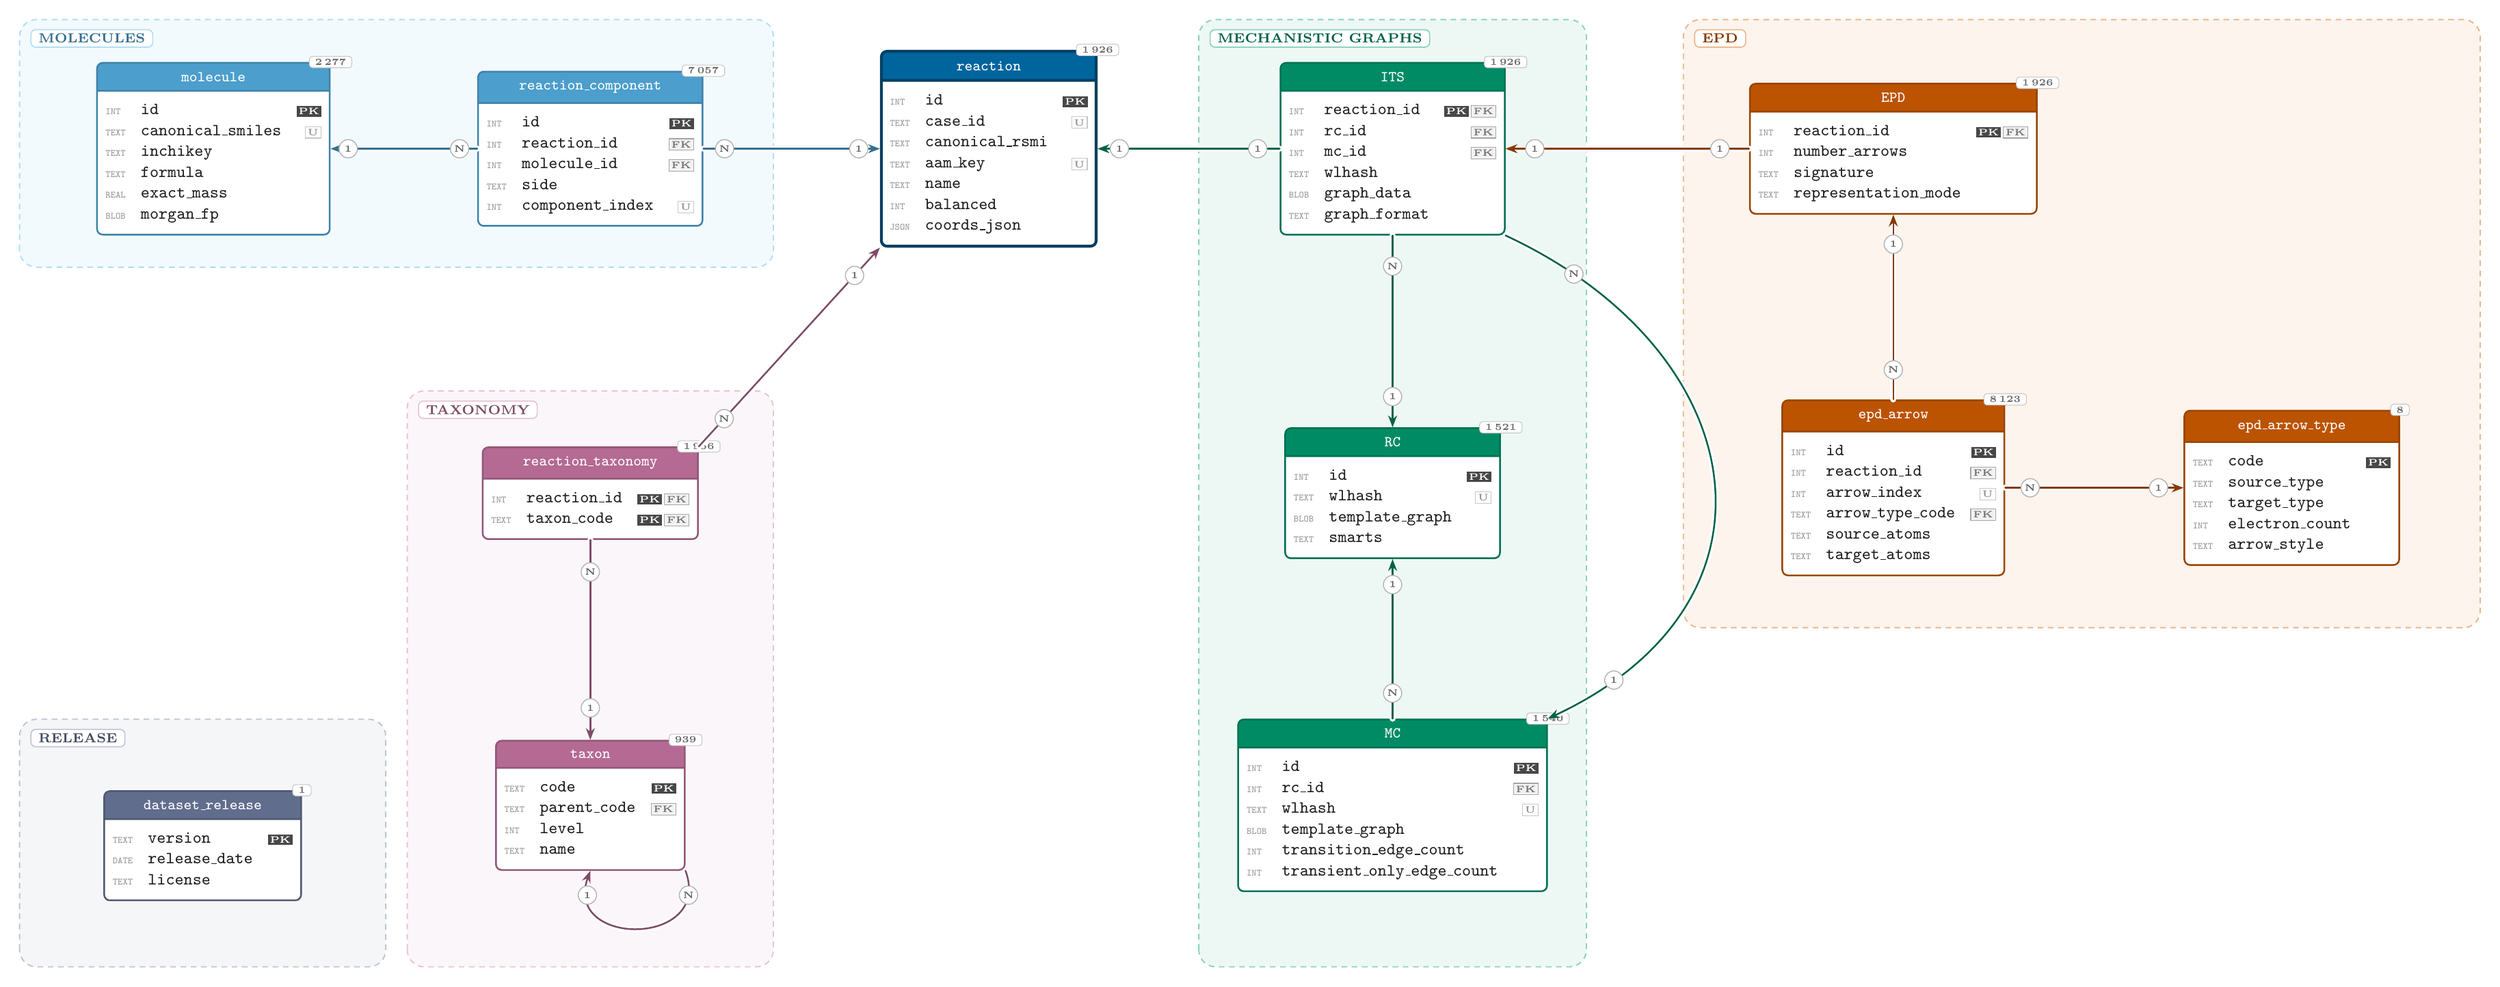
\begin{tikzpicture}[
  font=\footnotesize, >=Latex, line cap=round, line join=round,
  % --- entity card ---
  er/.style={rectangle split, rectangle split parts=2, draw=#1!72!black,
    line width=0.9pt, rounded corners=3pt, inner sep=4.5pt,
    rectangle split part fill={#1!88!black,white}, rectangle split part align=base},
  % --- the reaction hub gets a heavier rim ---
  hub/.style={er=#1, line width=1.5pt, draw=#1!55!black},
  % --- foreign-key edge; white halo keeps it legible on dark backgrounds ---
  rel/.style={-{Stealth[length=2.2mm]}, draw=black!55, line width=0.9pt,
    rounded corners=3pt,
    preaction={draw=white, line width=3.2pt, line cap=round}},
  relc/.style={rel, draw=#1!62!black},
  % --- cardinality bubble ---
  card/.style={circle, fill=white, draw=black!30, line width=0.5pt,
    font=\tiny\bfseries, text=black!62, inner sep=0.3pt, minimum size=3.4mm},
  % --- row-count chip pinned to a card corner ---
  chip/.style={fill=white, draw=black!22, rounded corners=1.6pt,
    inner xsep=3pt, inner ysep=1.4pt, font=\tiny\bfseries, text=black!58},
  % --- layer panel + its tag ---
  panel/.style={rounded corners=9pt, fill=#1!7, draw=#1!45, line width=0.7pt,
    dash pattern=on 3pt off 2.4pt},
  ptag/.style={fill=white, draw=#1!45, line width=0.6pt, rounded corners=2.5pt,
    inner xsep=4pt, inner ysep=2.2pt, font=\scriptsize\bfseries,
    text=#1!62!black, anchor=west},
]

% =====================================================================
%  layer panels (drawn behind the cards)
% =====================================================================
\begin{scope}[on background layer]
  \draw[panel=cProv]  (-17.6,-11.6) rectangle (-10.8, -7.0);
  \draw[panel=cMol]   (-17.6,  1.4) rectangle ( -3.6,  6.0);
  \draw[panel=cTax]   (-10.4,-11.6) rectangle ( -3.6, -0.9);
  \draw[panel=cGraph] (  4.3,-11.6) rectangle ( 11.5,  6.0);
  \draw[panel=cEPD]   ( 13.3, -5.3) rectangle ( 28.1,  6.0);
\end{scope}

\node[ptag=cProv]  at (-17.4,-7.35) {RELEASE};
\node[ptag=cMol]   at (-17.4,  5.65) {MOLECULES};
\node[ptag=cTax]   at (-10.2, -1.25) {TAXONOMY};
\node[ptag=cGraph] at (  4.5,  5.65) {MECHANISTIC GRAPHS};
\node[ptag=cEPD]   at ( 13.5,  5.65) {EPD};

% =====================================================================
%  release provenance
% =====================================================================
\node[er=cProv] (drel) at (-14.2,-9.35)
  {\ttl{dataset\_release}\nodepart{two}\DB{%
    \Rw{TEXT}{version}{\pk}\Rw{DATE}{release\_date}{}\Rw{TEXT}{license}{}}};
\node[chip] at (drel.north east) {1};

% =====================================================================
%  molecular structure
% =====================================================================
\node[er=cMol] (mol) at (-14.0,3.6)
  {\ttl{molecule}\nodepart{two}\DB{%
    \Rw{INT}{id}{\pk}\Rw{TEXT}{canonical\_smiles}{\uq}\Rw{TEXT}{inchikey}{}%
    \Rw{TEXT}{formula}{}\Rw{REAL}{exact\_mass}{}\Rw{BLOB}{morgan\_fp}{}}};
\node[chip] at (mol.north east) {2\,277};

\node[er=cMol] (comp) at (-7.0,3.6)
  {\ttl{reaction\_component}\nodepart{two}\DB{%
    \Rw{INT}{id}{\pk}\Rw{INT}{reaction\_id}{\fk}\Rw{INT}{molecule\_id}{\fk}%
    \Rw{TEXT}{side}{}\Rw{INT}{component\_index}{\uq}}};
\node[chip] at (comp.north east) {7\,057};

% =====================================================================
%  reaction hub
% =====================================================================
\node[hub=cRxn] (rxn) at (0.4,3.6)
  {\ttl{reaction}\nodepart{two}\DB{%
    \Rw{INT}{id}{\pk}\Rw{TEXT}{case\_id}{\uq}\Rw{TEXT}{canonical\_rsmi}{}%
    \Rw{TEXT}{aam\_key}{\uq}\Rw{TEXT}{name}{}\Rw{INT}{balanced}{}%
    \Rw{JSON}{coords\_json}{}}};
\node[chip] at (rxn.north east) {1\,926};

% =====================================================================
%  classification & ontology
% =====================================================================
\node[er=cTax] (rtax) at (-7.0,-2.8)
  {\ttl{reaction\_taxonomy}\nodepart{two}\DB{%
    \Rw{INT}{reaction\_id}{\pkfk}\Rw{TEXT}{taxon\_code}{\pkfk}}};
\node[chip] at (rtax.north east) {1\,956};

\node[er=cTax] (tax) at (-7.0,-8.6)
  {\ttl{taxon}\nodepart{two}\DB{%
    \Rw{TEXT}{code}{\pk}\Rw{TEXT}{parent\_code}{\fk}\Rw{INT}{level}{}%
    \Rw{TEXT}{name}{}}};
\node[chip] at (tax.north east) {939};

% =====================================================================
%  mechanistic graph layer
% =====================================================================
\node[er=cGraph] (its) at (7.9,3.6)
  {\ttl{ITS}\nodepart{two}\DB{%
    \Rw{INT}{reaction\_id}{\pkfk}\Rw{INT}{rc\_id}{\fk}\Rw{INT}{mc\_id}{\fk}%
    \Rw{TEXT}{wlhash}{}%
    \Rw{BLOB}{graph\_data}{}\Rw{TEXT}{graph\_format}{}}};
\node[chip] at (its.north east) {1\,926};

\node[er=cGraph] (rc) at (7.9,-2.8)
  {\ttl{RC}\nodepart{two}\DB{%
    \Rw{INT}{id}{\pk}\Rw{TEXT}{wlhash}{\uq}\Rw{BLOB}{template\_graph}{}%
    \Rw{TEXT}{smarts}{}}};
\node[chip] at (rc.north east) {1\,521};

\node[er=cGraph] (mc) at (7.9,-8.6)
  {\ttl{MC}\nodepart{two}\DB{%
    \Rw{INT}{id}{\pk}\Rw{INT}{rc\_id}{\fk}\Rw{TEXT}{wlhash}{\uq}%
    \Rw{BLOB}{template\_graph}{}\Rw{INT}{transition\_edge\_count}{}%
    \Rw{INT}{transient\_only\_edge\_count}{}}};
\node[chip] at (mc.north east) {1\,540};

% =====================================================================
%  electron-pushing description layer
% =====================================================================
\node[er=cEPD] (epd) at (17.2,3.6)
  {\ttl{EPD}\nodepart{two}\DB{%
    \Rw{INT}{reaction\_id}{\pkfk}\Rw{INT}{number\_arrows}{}%
    \Rw{TEXT}{signature}{}\Rw{TEXT}{representation\_mode}{}}};
\node[chip] at (epd.north east) {1\,926};

\node[er=cEPD] (arr) at (17.2,-2.7)
  {\ttl{epd\_arrow}\nodepart{two}\DB{%
    \Rw{INT}{id}{\pk}\Rw{INT}{reaction\_id}{\fk}\Rw{INT}{arrow\_index}{\uq}%
    \Rw{TEXT}{arrow\_type\_code}{\fk}\Rw{TEXT}{source\_atoms}{}%
    \Rw{TEXT}{target\_atoms}{}}};
\node[chip] at (arr.north east) {8\,123};

\node[er=cEPD] (atype) at (24.6,-2.7)
  {\ttl{epd\_arrow\_type}\nodepart{two}\DB{%
    \Rw{TEXT}{code}{\pk}\Rw{TEXT}{source\_type}{}\Rw{TEXT}{target\_type}{}%
    \Rw{INT}{electron\_count}{}\Rw{TEXT}{arrow\_style}{}}};
\node[chip] at (atype.north east) {8};

% =====================================================================
%  foreign-key edges  (child -> parent)
% =====================================================================
% structure
\draw[relc=cMol] (comp.west) -- (mol.east)
  node[card,pos=0.12]{N} node[card,pos=0.88]{1};
\draw[relc=cMol] (comp.east) -- (rxn.west)
  node[card,pos=0.12]{N} node[card,pos=0.88]{1};

% classification
\draw[relc=cTax] (rtax.north east) -- (rxn.south west)
  node[card,pos=0.14]{N} node[card,pos=0.86]{1};
\draw[relc=cTax] (rtax.south) -- (tax.north)
  node[card,pos=0.16]{N} node[card,pos=0.84]{1};
\draw[relc=cTax] (tax.south east) to[out=-70,in=-110,looseness=2.2]
  node[card,pos=0.12]{N} node[card,pos=0.88]{1} (tax.south);

% mechanistic graphs
\draw[relc=cGraph] (its.west) -- (rxn.east)
  node[card,pos=0.12]{1} node[card,pos=0.88]{1};
\draw[relc=cGraph] (its.south) -- (rc.north)
  node[card,pos=0.16]{N} node[card,pos=0.84]{1};
\draw[relc=cGraph] (mc.north) -- (rc.south)
  node[card,pos=0.16]{N} node[card,pos=0.84]{1};
\draw[relc=cGraph] (its.south east) to[out=-25,in=25,looseness=1.45]
  node[card,pos=0.10]{N} node[card,pos=0.90]{1} (mc.north east);

% electron pushing
\draw[relc=cEPD] (epd.west) -- (its.east)
  node[card,pos=0.12]{1} node[card,pos=0.88]{1};
\draw[relc=cEPD] (arr.north) -- (epd.south)
  node[card,pos=0.16]{N} node[card,pos=0.84]{1};
\draw[relc=cEPD] (arr.east) -- (atype.west)
  node[card,pos=0.14]{N} node[card,pos=0.86]{1};
\end{tikzpicture}
\end{document}
